% !TeX program = xelatex
%吉林大学通信工程学院自动化毕业设计latex模版
%525寝室专用版
\documentclass[12pt,a4paper,openany,oneside]{book}%正文小四
\usepackage{emptypage}
\usepackage{fancyhdr}  %页眉页脚
\usepackage{tocloft}	%目录格式
\usepackage{titlesec}
\usepackage{indentfirst} % 首段缩进
\usepackage{amsmath,amsthm,amssymb,appendix,bm,graphicx,hyperref,mathrsfs}
\usepackage[heading=true]{ctex}
\usepackage{titletoc}
\usepackage{pdfpages}
\usepackage{enumitem}
\usepackage{graphicx}
\usepackage{caption}
\usepackage{booktabs}
\usepackage{tabularx}
\usepackage{array}
\usepackage{float}
\usepackage{graphicx}
\usepackage{subcaption}
\usepackage[margin=1in]{geometry}
\usepackage[sort&compress]{gbt7714}   % 可选参数含义：存在多篇引文时自动压缩序号
\usepackage{makecell}
\usepackage{tabularx}
\usepackage{array}
\hypersetup{
	colorlinks=true,
	linkcolor=black,
	citecolor=black
}%隐藏超链接跳转红框、论文引用绿框
%-------------------目录字号格式设定--------------------------
\renewcommand{\contentsname}{\heiti\zihao{3}目\ \   \heiti\zihao{3}录}
% 设置目录样式
\titlecontents{chapter}[0em]{\songti\zihao{4}}{\thecontentslabel\quad}{}{\titlerule*[1pc]{.}\contentspage}[\addvspace{0pt}]
\renewcommand{\cftchapfont}{\songti\zihao{4}} % 章节目录字体为宋体四号
\renewcommand{\cftchappagefont}{\songti\zihao{4}} % 章节目录页码字体为宋体四号
\setlength{\cftbeforechapskip}{-8pt} % 章节目录之前的垂直间距为0pt

% 设置一级目录
\renewcommand{\cftsecfont}{\songti\zihao{4}} % 一级目录字体为宋体四号
\renewcommand{\cftsecpagefont}{\songti\zihao{4}} % 一级目录页码字体为宋体四号
\setlength{\cftsecindent}{1em} % 一级目录左缩进一个字符
\setlength{\cftbeforesecskip}{0.8pt} % 一级目录之前的垂直间距为0pt

% 隐藏二级目录
\setcounter{tocdepth}{1} % 设置目录深度为1，只显示chapter和section





% --------目录格式设置第一页页码与全局格式一致-------------
\usepackage{tocloft}
\tocloftpagestyle{fancy}

%------行距与缩进设置------
\usepackage{indentfirst} % 设置首行缩进
\usepackage{setspace} % 设置行距
\setlength{\parindent}{2em} % 设置首行缩进为2个字符的宽度
\setstretch{1.5}

%------字体设置------
\usepackage{ctex} % 设置中文字体
\usepackage{fontspec} % 设置英文字体
\setCJKmainfont[AutoFakeBold=1.5,AutoFakeSlant=.4]{宋体}
\setmainfont{Times New Roman}

%------页边距，每页限定41行------
\usepackage{geometry}
\geometry{top=2.3cm, bottom=2.8cm, left=3.35cm, right=2.5cm}
%\newcommand{\linesperpage}{39} % 每页行数
%\setlength{\textheight}{\linesperpage\baselineskip}

%------标题------
\title{\textbf{冗余机械臂的力-位混合控制系统设计}}

%------标题格式------
\ctexset{section={
		format+=\raggedright\zihao{4},
		beforeskip=5pt,
		afterskip=5pt,
	},
	subsection={
		format+=\zihao{-4},
		beforeskip=5pt,
		afterskip=5pt
	},
	chapter={
		format+=\zihao{-3}\bfseries,
		number = \arabic{chapter},
		beforeskip=-15pt,
		afterskip=15pt
	}
}

%----------图表、公式按章节编号----------
\numberwithin{equation}{chapter}%公式按章节编号
\numberwithin{figure}{chapter}%图表按章节编号
\captionsetup[figure]{font={small,bf,stretch=1.25}, labelsep=space} %字体设为small（对应五号字体)\bf加粗\stretch1.25倍行距\space去分号
\captionsetup[table]{font={small,bf,stretch=1.25}, labelsep=space}
\renewcommand{\theequation}{\arabic{chapter}.\arabic{equation}}%公式中间用“ - ”连接
\renewcommand{\thetable}{\thechapter{}-\arabic{table}}%图表中间用“ - ”连接
\renewcommand{\thefigure}{\thechapter{}-\arabic{figure}}
%----------参考文献的标号设置为方括号且为上标----------
\makeatletter
\def\@cite#1#2{\textsuperscript{[{#1\if@tempswa , #2\fi}]}}
\makeatother

%----------页眉设置----------
\pagestyle{fancy}
\fancyhf{} % 清除当前设置的页眉页脚
\fancyfoot[C]{\zihao{5} — \hspace{0.25em} \thepage \hspace{0.25em} —} % 设置页脚中间显示页码
\fancyhead[C]{\nouppercase{\zihao{-5} \leftmark}} % 设置页眉中间为章节标题和编号，应用小五号字体大小
\renewcommand{\headrulewidth}{0.4pt}
\renewcommand{\footrulewidth}{0pt}
\fancypagestyle{plain}{
	\fancyhf{}
	\fancyhead[C]{\nouppercase{\zihao{-5} \leftmark}} % 特殊页也显示页眉
	\fancyfoot[C]{\zihao{5}— \hspace{0.25em} \thepage \hspace{0.25em} —}
	\renewcommand{\headrulewidth}{0.4pt} % 页眉下方横线也显示
}
\renewcommand{\chaptermark}[1]{\markboth{第 \thechapter\ 章\ #1}{}}
\fancypagestyle{tocstyle}{
	\fancyhf{}
	\fancyhead[C]{\nouppercase{\fontsize{12pt}{14pt}\selectfont \zihao{-5}目录}} % 目录页特有的页眉
	\fancyfoot[C]{\zihao{-5}— \hspace{0.25em} \thepage \hspace{0.25em} —}
	\renewcommand{\headrulewidth}{0.4pt}
}
% 图片 --- 图片路径，图片标题，图片引用名,图片宽度
\newcommand{\insertfig}[4]{
    \begin{figure}[h] %H为当前位置，!htb为忽略美学标准，htbp为浮动图形
        % 图片与上下文的间距
        \setlength{\intextsep}{10pt}
        \setlength{\belowcaptionskip}{0cm} %调整图片标题与下文距离
        \centering %图片居中
        \includegraphics[width=#4]{#1} %插入图片，[]中设置图片大小，{}中是图片文件名
        \caption{#2} % 最终文档中希望显示的图片标题
        \label{#3} % 用于文内引用的标签
    \end{figure}
}
%---------------------------------------------------
%-------------------以下是文章部分-------------------
%---------------------------------------------------
\begin{document}
	%----------封面设置，将封面单页pdf命名后放在当前文件夹下----------
	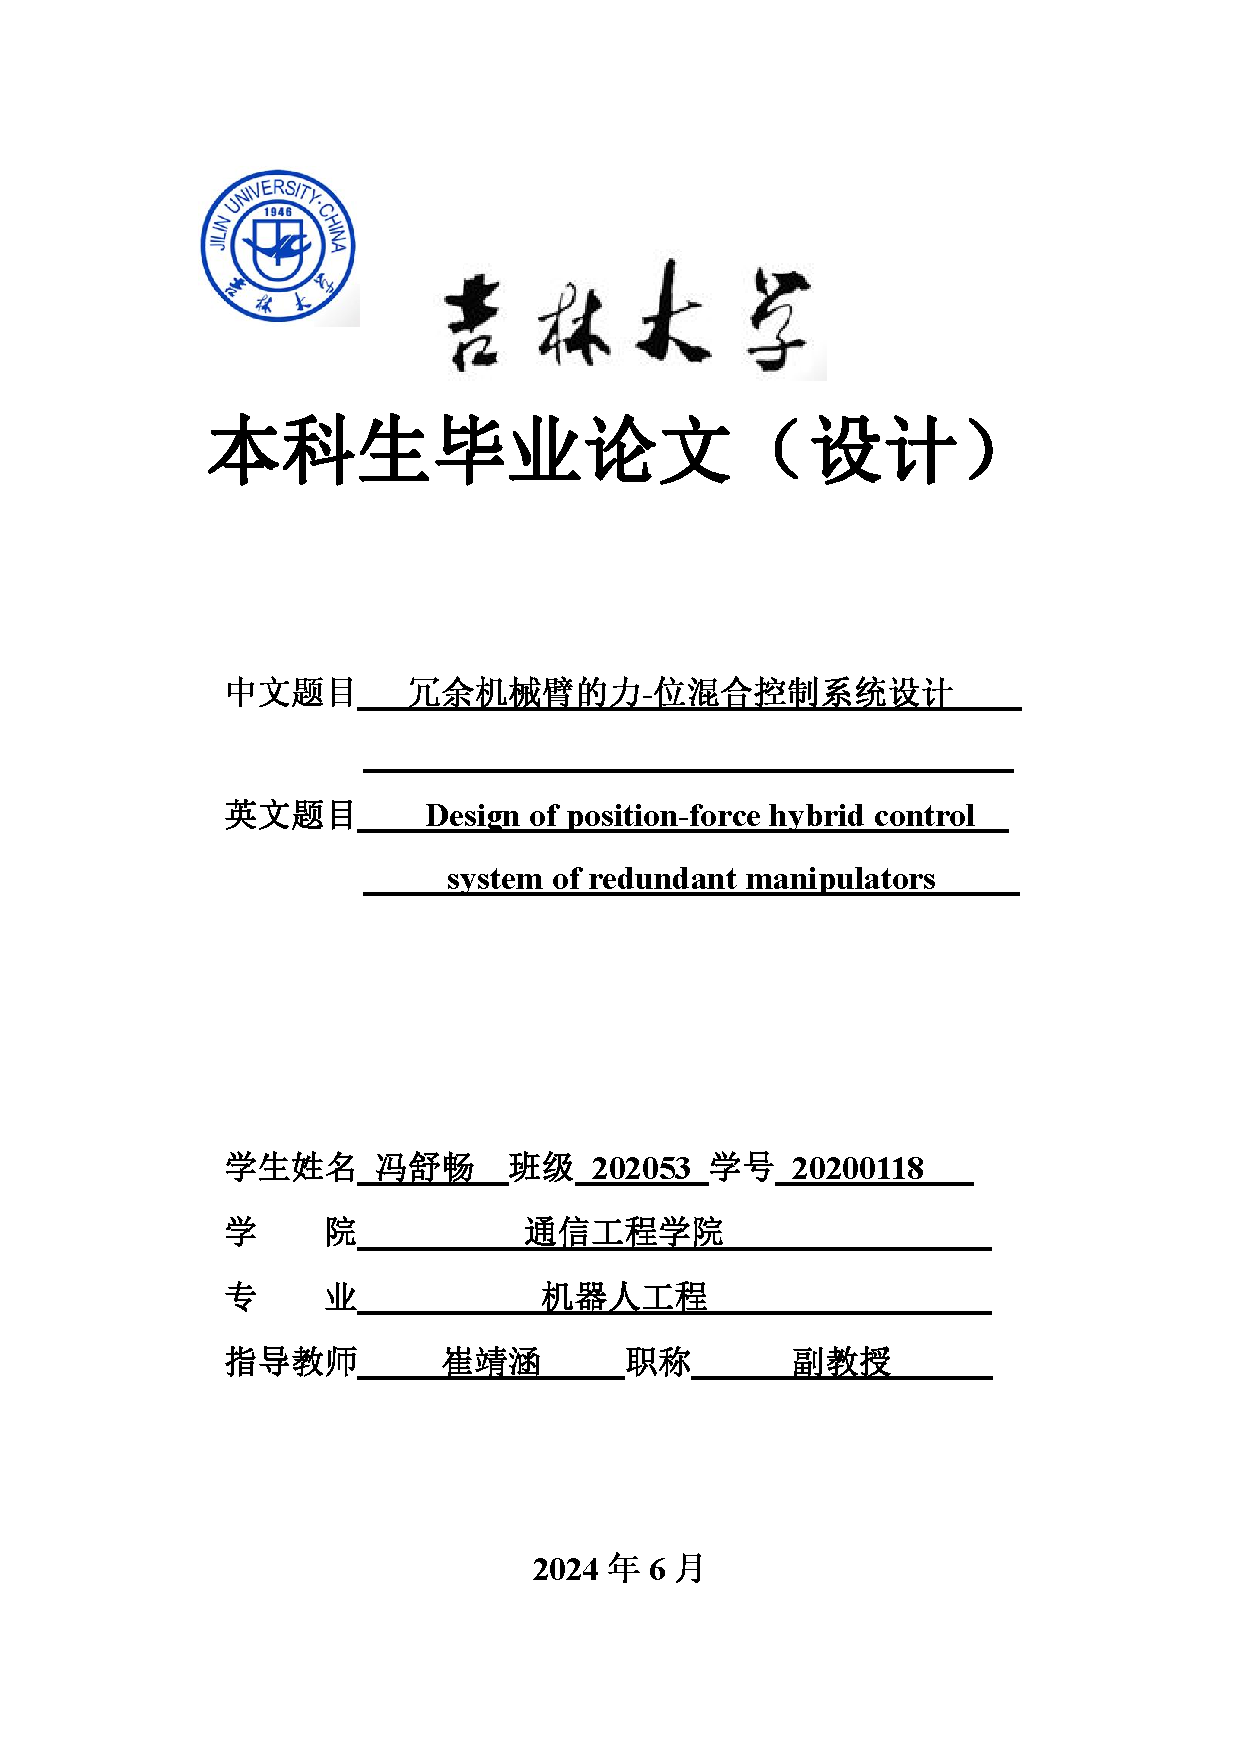
\includepdf[pages=-]{cover.pdf}
	\clearpage
	
\includepdf[pages=-]{cns.pdf}
	\newpage
	
\includepdf[pages=-]{sqs.pdf}
	\newpage
	\pagenumbering{Roman}
	\setcounter{page}{3}
	\markboth{摘要}{}
	\begin{center}
		\textbf{\fontsize{16}{18}\selectfont \zihao{-3}摘\ \ 要}
	\end{center}
	%---------摘要正文------
	
	随着工业机器人相关技术的进步以及机器人应用环境的拓宽，人们从机械臂的结构上寻求突破，冗余机械臂得到了更广泛的研究。同时随着机器人的任务复杂性增加，对机器人仅进行位置控制已经不足够完成任务。本课题设计了冗余机械臂的力-位混合控制系统，以冗余机械臂为被控对象，控制目的是使其末端执行器输出准确的位置和接触力。具有广阔的应用场景和重要的实际意义。本文涉及到机械臂本体建模技术，力位混合控制技术，主要工作如下：\par
(1)完成了机械臂模型的建立。首先选取机械臂模型，用改进D-H参数法进行运动学建模，推导正运动学关系，然后计算雅可比矩阵和力域中的雅可比矩阵，实现关节空间和笛卡尔空间的转换，得到控制量与被控量的关系。最后在MATLAB软件上进行仿真，验证机械臂运动学的正确性。\par
(2)进行了力-位混合控制算法的研究。首先将控制任务解耦为互相正交的位置子空间和力子空间，设计力环与位置环的控制，然后对此设计PID控制器，最后进行多种仿真任务，在MATLAB上进行仿真实验，调整PID参数，验证算法的正确性和有效性。
	\\ \textbf{\fontsize{16}{18}\selectfont \zihao{-4}关键字：}冗余机械臂；力位混合控制；PID控制器
	
	
	
	
	
	
	\newpage
	\markboth{ABSTRACT}{}
	\begin{center}
		\textbf{\fontsize{16}{18}\selectfont \zihao{-3}ABSTRACT}
	\end{center}
	%--------英文摘要------
	
	With the advancement of industrial robot related technologies and the expansion of robot application environment, people seek breakthroughs in the structure of robot manipulators,redundant manipulators have thus been widely studied. At the same time, with the increasing complexity of robot tasks, position control alone is no longer sufficient to complete the task. This paper designs a force-position hybrid control system for redundant manipulators. The redundant manipulator is used as the controlled plant, and the control purpose is to make its end effector output accurate position and contact force. It has a wide range of application scenarios and important practical significance. This paper involves manipulator body modeling technology and force-position hybrid control technology. The main work is as follows:

(1) The establishment of the manipulator model was completed. First, the manipulator model was selected, and the kinematic modeling was performed using the improved D-H parameter method to derive the positive kinematic relationship. Then, the Jacobian matrix and the Jacobian matrix in the force domain were calculated to realize the conversion between the joint space and the Cartesian space, and the relationship between the control quantity and the controlled quantity was obtained. Finally, simulation was performed on MATLAB software to verify the correctness of the manipulator kinematics.

(2) The force-position hybrid control algorithm was studied. First, the control task is decoupled into orthogonal position subspace and force subspace, and the control of the force loop and position loop is designed. Then, design a PID controller and adjust its parameters. Finally,various simulation tasks are performed and simulation experiments are conducted on MATLAB to verify the correctness and effectiveness of the algorithm.
	\\ \textbf{\fontsize{16}{18}\selectfont \zihao{-4}Keywords：}Redundant manipulator;force-position hybrid control;PID controller
	
	
	
	
	
	
	
	%---------目录-------------
	\newpage
	\begin{center}
		\vspace*{-2.5cm} % 调整标题与页眉的间距
		\tableofcontents	
		\thispagestyle{tocstyle}
		\addtocontents{toc}{\vspace{-12mm}}

	\end{center}
    \clearpage
	\pagenumbering{arabic}
	\setcounter{page}{1}
	%-----------论文正文-----------
\chapter{绪论}
	本章根据本毕业设计研究的内容、背景以及意义，说明了冗余机械臂与力位控制算法在实际生产生活中的应用以及其重要的工程与研究意义，并且对目前关于冗余机械臂以及力位置控制算法的国内外现状进行介绍。最后阐述了本文是如何设计冗余机械臂的力位混合控制系统对末端执行器进行准确的位置控制和接触力控制，并介绍了本文的主要内容的结构。
\section{研究背景及意义}
伴随全球数字化进程加速，机器人产业正迎来关键爆发时刻，众多机器人技术取得重大突破，推动了人类生产力的极大进步。机器人作为制造业的璀璨明珠，是衡量一个国家科技创新能力和高端制造业水平的重要标志之一。我国高度重视机器人行业的发展，2023年1月，工业和信息化部等十六部门联合印发《“机器人+”应用行动实施方案》，深化重点领域“机器人+”应用，增强“机器人+”应用基础支撑能力。我国具有广阔的机器人应用市场，拥有较雄厚的机器人产业实力。据中国电子学会预计，2023年全球机器人市场规模已达将近336亿美元，我国机器人市场规模可达839亿元人民币，在全球市场中占比达到53\%，装机量在全球占比将达到50\%以上。这反映出我国具有巨大的机器人研究潜力以及广阔的机器人消费市场。

冗余机械臂是先进机器人领域的重要研究方向，冗余指的是其在结构设计方面有着额外的自由度，其拥有的自由度大于完成控制任务所必须的自由度，这使得冗余机械臂相比于非冗余机械臂，有着更优秀的灵活性、鲁棒性、快速性与准确性\cite{r1}。因为机械臂冗余的自由度使其能够以更多关节姿态到达指定位置或者沿轨迹运动，使得冗余机械臂具有本体避障\cite{r2}，避开奇异点\cite{r3}，避开关节限位等与生俱来的优势。因此，冗余机械臂更适用于复杂、狭小的动态工作环境，正是由于这些优势，冗余机械臂在航空航天、社会服务、工业制造等大量领域中的研究与应用愈加广泛。

随着机器人应用领域的扩展，机械臂的工作任务越来越多的从非接触作业中的单一的位置输出轨迹跟踪到了接触作业中的需要与机械臂的工作环境进行交互。此时，纯粹的位置控制已经不能满足任务的需要。例如在零件装配、磨削、抛光作业\cite{r4}\cite{r5}等场景中，机械臂末端微小的位置误差可能导致巨大的力变化，所以要求机械臂能够对接触力进行精确控制，对于机械臂末端同时进行力控制研究，能弥补位置控制的不足\cite{r6}，对于高效安全的完成工作任务具有重要意义。接触作业是机器人应用的重要领域，焊接机器人、装配机器人、机械加工机器人发展迅速。例如2016-2021年我国焊接机器人市场销量从2.84万台增长至4.85万台，年复合增速为17\%，2021年我国焊接机器人系统集成市场规模达210.4亿元。

人形机器人是如今机器人行业中的火爆领域，百度、阿里、腾讯、小米等大公司都开始投资了人形机器人企业或者自研人型机器人。人形机器人有着仿人结构，也有着与人类一样冗余的自由度设计。同时人形机器人也需要像人一样不仅能够顺滑地使手指末端精准地沿指定轨迹运动，还要对环境施加准确的力。例如无论是特斯拉第二代人形机器人擎天柱Optimus Gen2用手指捏起鸡蛋(如图\ref{Fig_optimus}），还是优必选人形机器人Walker S收纳桌面并将橙子递给李彦宏(如图\ref{Fig_WalkerS})，都需要对机器人进行力和位置两方面同时控制。精确的力控制与位置控制能够使得冗余机械臂具有出色的环境适应能力和拟人化工作能力。因此设计针对冗余机械臂的力位混合控制系统尤为重要，有利于机器人实现更多样的功能。
\begin{figure}[h]
  \centering
  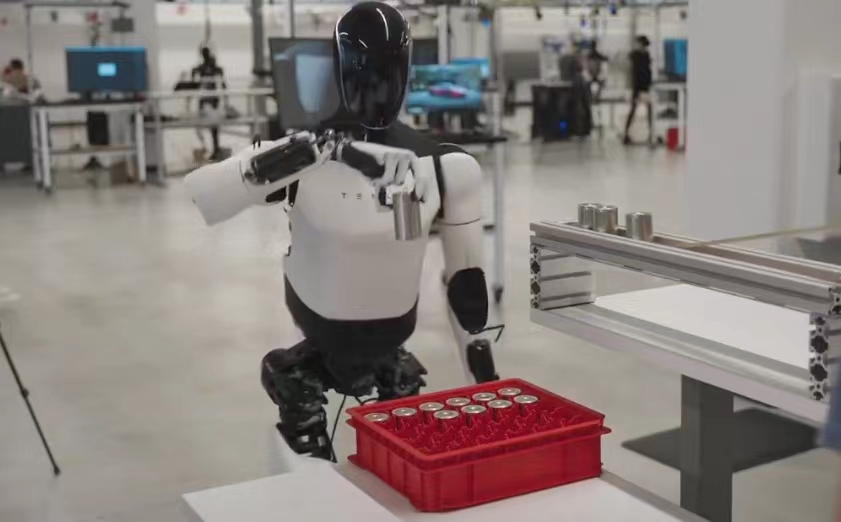
\includegraphics[width=10cm]{figures/optimus.jpg}
  \caption{特斯拉optimus机器人在整理电池}\label{Fig_optimus}
\end{figure}
\begin{figure}[h]
  \centering
  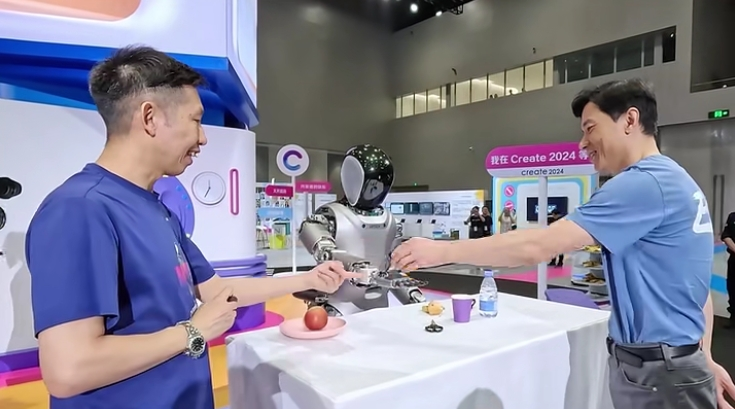
\includegraphics[width=10cm]{figures/递橙子.png}
  \caption{Walker S在给李彦宏递橙子}\label{Fig_WalkerS}
\end{figure}
对于冗余机械臂的力位置混合控制是一个复杂的问题，对冗余机械臂的建模要比非冗余机械臂的建模要困难许多。增加的自由度会使机械臂运动学和动力学的模型更为复杂，计算量也会增加许多。尤其是在逆运动学方面，某个位置解一般会对应多个关节空间的关节逆解。在力位混合控制方面，需要对控制任务进行解耦至子空间，并且分别研究位置控制规律与力控制规律，建立分别的控制通道，保证它们相对独立又能将控制量同时施加在执行器上。对冗余机械臂的力位混合控制研究对机械臂能正常完成任务具有基础性意义。
\section{国内外研究现状}
本节旨在介绍与本文研究相关的技术与发展成果，主要包括对于冗余机械臂的研究与对力位混合控制的研究，下文将分别阐述其相关的研究现状。
\subsection{冗余自由度机器人的发展现状}
早在上世纪60年代至70年代，生产中对于工业自动化的需求增长，尤其在汽车制造业中，初期的多关节机器人开始出现，但是大多具有较少自由度，主要用于重复性作业。随着计算机技术与控制理论的发展，拥有复杂结构的机械臂得以实现与应用，包括增加关节以达到更多自由度的设计。\par
为了抢占工业智能化制高点，德国在2013年提出了工业4.0战略，开启了新一轮的工业转型。在2014年11月，德国的机器人制造巨头KUKA在中国国际工业博览会上首次展示了KUKA第一款七自由度机器人LBR iiwa(如图\ref{Fig_iiwa})，是一款高灵活性的轻敏机器人。2016年，KUKA又推出了全球首款认证的医疗机器人LBR Med，这款机器人可以使用各种医疗工具进行多种外科与骨科诊疗。2015年4月的汉诺威工业博览会上，瑞士ABB公司的双臂工业机器人YuMi首次亮相，YuMi的双臂结构共包含了14个自由度,能实现人机协作。2023年12月，Tesla推出第二代Optimus，它光是手掌就有11个自由度，能灵巧完成拿鸡蛋，叠衬衫等任务。
%\insertfig{./figures/iiwa.jpg}{KUKA七自由度机器人LBR iiwa}{Fig_iiwa}{4cm}
\begin{figure}[h]
  \centering
  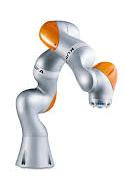
\includegraphics[width=4cm]{figures/iiwa.jpg}
  \caption{KUKA七自由度机器人LBR iiwa}\label{Fig_iiwa}
\end{figure}

我国对冗余机器臂的科研工作起步较晚，在20世纪90年代初国家“863”计划、国家自然科学基金的资助下，多家单位开始冗余机械臂的研究。机器人技术专家张启先院士课题组，首先研制出了国内首台七自由度冗余机械臂。在2015年11月中国国际工业博览会上，沈阳新松机器人公司推出了中国首款量产的七自由度协作机器人，它具备牵引示教、碰撞检测、快速配置、视觉引导等功能，在布局紧凑、精度要求高的柔性化生产线上发挥重要作用。浙江人形机器人创新中心发布了“领航者1号”机器人(如图\ref{Fig_lhz})，拥有39个自由度和多自由度灵巧手，多自由度灵巧手有15个手指关节，6个主动自由度。
%\insertfig{./figures/lhz1.png}{领航者1号机器人}{Fig_lhz}{10cm}
\begin{figure}[h]
  \centering
  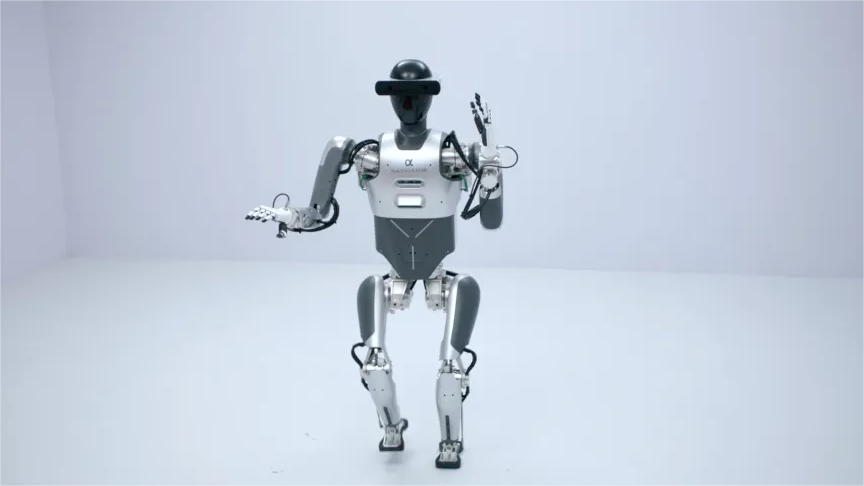
\includegraphics[width=10cm]{figures/lhz1.png}
  \caption{领航者1号机器人}\label{Fig_lhz}
\end{figure}

机械臂的冗余特性赋予了机械臂灵活性，也增强了实现次要目标的能力，但也给数学上解运动学和动力学，尤其是逆运动学冗余解析方面带来了困难。文献\cite{r7}提出了一种选择最优关节角参数的位置级逆运动学优化算法，结合牛顿迭代法拉格朗日乘子法，将机械臂最优构型的计算问题转化为机械臂最优标志参数的寻根问题。文献\cite{r8}提出了一种基于迭代优化和神经网络补偿的半参数动力学模型辨识方法，使用遗传算法与两层循环网络对动力学模型进行精确辨识。文献\cite{r9}引入臂角参数建立了逆解的解析解公式，通过自适应权重参数调节任务优先级，并引入粒子群优化算法得出最优解。文献\cite{r10}提出了一种利用增广雅可比矩阵的逆运动学求解算法，使系统满足实时控制的要求且能够保证机械臂追踪封闭轨迹时运动的可重复性。文献\cite{r11}将冗余解析求解问题转化为约束下的最优化问题,将次级任务作为目标函数，将主要任务与物理约束作为约束条件。文献\cite{r111}通过坐标系转换的方式将交互设备屏幕坐标进行变换实现触控交互,并通过柱面避障运动规划,解决了冗余自由度机械臂运动控制中人机交互性不强、避障算法较为复杂且躲避非结构化障碍较为困难的问题。文献\cite{r112}针对冗余机械臂对应目标位置的轨迹跟踪性能难以优化的问题，研究了基于粒子群优化算法的冗余机械手轨迹跟踪方法，推导冗余机械臂末端运动轨迹方程，利用伪逆雅可比矩阵求解机械手冗余问题。并结合粒子群优化算法，得到冗余机械手整体轨迹的最优跟踪结果，具有较高的跟踪精度和可靠性。

\subsection{力位置控制的研究现状}
国内外学者对力-位置控制的研究可以总结为两类，一是机器人的阻抗控制\cite{r12}，二是力-位置混合控制\cite{r13}。阻抗控制对机器人和环境之间的接触力控制是间接的，阻抗控制需要获取环境参数，建立作用力与位置误差之间的物理模型。在机器人与外界环境交互过程中，由于各种干扰的存在与精度的限制，误差是不可避免的，阻抗控制需要使机器人有合适的阻尼系数，通过控制末端的位移从而控制与环境的作用力。文献\cite{r131}设计了阻抗参数在线调整与离线优化的自适应阻抗控制算法，实现了打磨力控制,针对阻尼参数和惯性参数难以整定的问题，以降低系统超调量和调整时间作为优化目标，采用改进粒子群算法进行阻抗参数离线优化，可以综合改善机器人的恒力控制性能。文献\cite{r132}把模糊逻辑控制器与阻抗控制器相合，使阻抗控制参数能随实际工况而变化,实现了变阻抗控制,改进了机器人力跟踪的实时性、稳定性。

力-位置混合控制方法是在Mason提出的对力和位置进行同时控制的思想上发展而来。1981年Raibert和Craig发表了著名的《Hybrid Position/Force Control of Manipulators》，标志着力/位置混合控制理论的问世\cite{r13}。由于与平面的接触力和沿平面的运动是相互正交的，可以将机器人末端自由度在笛卡尔空间中分解，在不同的自由度进行力控制或者位置控制。
%\insertfig{./figures/hpf.png}{Craig教授提出的力/位置混合控制器}{Fig_hpf}{10cm}
\begin{figure}[h]
  \centering
  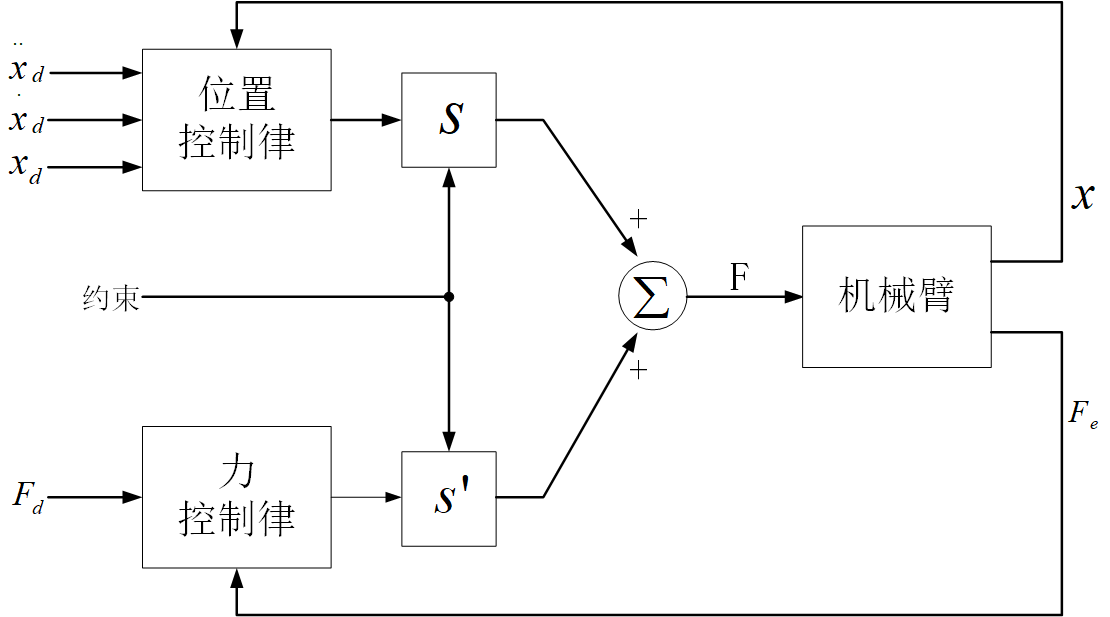
\includegraphics[width=10cm]{figures/hpf.png}
  \caption{Craig教授提出的力/位置混合控制器}\label{Fig_hpf}
\end{figure}

针对机器人的力位混合控制系统的设计可以大致分为基于经典控制理论和基于现代控制、智能控制理论两种方法。经典控制理论采用滑模控制、自适应控制、模型跟踪控制和鲁棒控制来减小系统动力学模型误差，提高对干扰和噪声的鲁棒性。文献\cite{r14}中，提出了一种鲁棒神经力控制方案。该控制器可以使机器人跟踪指定的期望力，同时可以补偿环境位置和刚度以及机器人动力学的不确定性。文献\cite{r15}提出了一种位置力控制策略，将机器人的运动完全解耦为两部分：控制末端执行器的运动以实现对环境的位置力控制，而内部运动则为旨在通过最小化冲击力来避开障碍物。文献\cite{r16}设计了存在未知扰动的自适应模糊力/位置混合控制方法，研究了仅依赖局部关节信息的模块化力/位置控制方法。文献\cite{r17}提出了一种用于多自由度机械臂的混合位置/力控制系统，设计了一种通过预测功能控制考虑扭矩约束的鲁棒系统。可以通过扰动观测器技术补偿了模型参数误差，并且即使扭矩饱和也可以执行适当的位置/力控制。文献\cite{r171}运用滑模控制原理，设计内外环控制通道，外环控制外部作用力和运动之间的阻抗关系，并向内环发出所需压力指令，内环进行压力跟踪控制表现自然柔顺性，达到了对于有界干扰保持全局渐进稳定的效果。文献\cite{r172}将操作器的动态模型转化为状态空间模型，并且将二次优化和滑模方法应用于机械臂的力位混合控制，由Hamilton Jacobi Bellman方法优化获得最佳控制律，该控制律是Lyapunov函数方法证明的全局指数稳定的。文献\cite{r173}设计同时考虑了不与环境或其他系统相互作用的无约束运动，以及系统与环境接触或与具有某些功能的另一个系统相互作用的约束运动，利用滑模控制实现机器人在两种环境下的自由切换，并且在减小控制器结构的变化的前提下保持系统的稳定性。文献\cite{r174}用设计了改进指数趋近律的滑模控制器和一种非线性滑模面的快速终端滑模控制器来控制绳驱动机械臂，该控制器在关节位置轨迹跟踪与振动抑制方面具备更优越的性能。

尽管以上采用经典控制理论的力位控制策略皆取得了不错的成果，但是都存在建模困难的问题，考虑到机器人的非线性和强耦合性质以及实际中力反馈的输入和不确定性，对机器人的建模和控制都增加了难度。

以机器学习、神经网络和模糊逻辑等为代表的智能控制算法针对系统的不确定性，研究人员提出了基于神经网络（NN）[包括径向基函数神经网络、模糊神经网络和循环神经网络（RNN）]的智能控制方法，用于处理系统的不确定性和扰动。文献\cite{r18}结合了循环技术和小波网络的优点针对一类移动机械臂，提出了一种基于模糊循环小波神经网络（RNN）的自适应力/运动控制方案。文献\cite{r181}用小波神经网络在环境动力学辨识中的优势，训练神经网络补偿机器人动力学参数变化，用神经网络对环境特征进行分类，降低机器人动力学模型的不确定性对系统的影响。文献\cite{r182}采用前馈神经网络来学习机器人动力学模型中存在的参数不确定性,刚性机械臂的力位混合控制设计基于神经网络的自适应控制方案。文献\cite{r183}设计了一种基于鲁棒自适应神经网络的混合位置/力控制方案，还开发了不需要扰动界限的先验信息的自适应补偿器，使机器人克服模型不确定性和外部干扰。文献\cite{r184}扩展了模糊控制，利用Desert\ Smarandache理论(DSmT)和中智逻辑集来提高步行机器人的动态稳定性。文献\cite{r185}设计了一种用于移动机器人的模糊逻辑控制器，可以处理外界环境的作用力并在环境干扰中保持机器人的平衡，该模糊逻辑控制器可以正确克服力的干扰并在移动机器人偏离预定轨迹时，让它们回到正确路径上。文献\cite{r186}提出了位置环境参数时的基于模糊神经网络的机器人力控制方法，采用遗传算法调整模糊神经网络的结构，使机器人能够较好地适应环境的变化。

智能控制算法中的神经网络的学习功能实现环境动力学参数调整与机器人模型参数补偿，模糊控制的不依赖模型，能做出最优适应性控制特点，保证了机器人力位控制中的实时性以及对偏差干扰的调整。然而上述工作大多以非冗余机械臂作为控制对象，针对冗余机械臂的控制研究与关注要少许多。

\section{主要研究内容与组织结构}
综上所述，无论是对冗余机械臂的研究还是对力位置混合控制算法的研究在理论与实际应用上都取得一定的成果，然而将两者结合起来，即对冗余机械臂进行力位混合控制的研究相对要少许多，并且在逆运动学的冗余解析方面，对于矩阵伪逆算法计算量较大。同时在机械臂实际运作过程中，应当使机械臂满足自身的物理约束，在自身关节限位的条件下完成任务。因此本文开展了针对冗余机械臂的力位混合控制系统设计研究，并使得其适用实际应用。论文主要研究内容如下：

1.冗余机械臂模型研究

冗余自由度机械臂的力-位混合控制系统建模，在仿真环境中为冗余机械臂采用D-H参数法建立运动学模型，用拉格朗日法建立动力学模型，方便后续的研究。

2.力位混合控制算法研究

将控制目标解耦为里控制环与位置控制环，依据运动学与动力学关系设计多输入多输出闭环系统各环节之间的数学关系。采用经典的PID算法，设计PID控制器，实现对机械臂末端执行器的高效控制。

本文共分五章，具体安排如下：\par
第1章为绪论，首先从研究背景与意义出发，概述了冗余机械臂和力位控制研究的发展过程与国内外研究现状，分析了目前研究取得的成就和存在的不足，列举了冗余机械臂和力位混合控制技术在机器人中的地位与应用，阐述了对冗余机械臂进行力位混合控制系统设计的实际意义与广阔前景。\par
第2章首先用Denavit–Hartenberg法对有冗余自由度机械臂进行前向运动学建模，根据机械臂参数计算关节角度的变化引起末端执行器在空间中的位置变化，然后基于拉格朗日法，根据机械臂的动能与势能进行动力学建模，得出机械臂的运动与驱动其运动的关节力矩之间的方程。最后求解速度雅可比矩阵与力雅可比矩阵，将关节转角与关节力矩分配至各个关节，得到笛卡尔空间和关节空间的转换关系。\par
第3章首先对力-位混合控制策略与算法展开研究，将控制任务解耦为子空间，研究子空间的控制规律，然后设计PID控制器对机械臂进行高效控制，使末端执行器输出精确的位置与接触力。\par
第4章首先搭建MATLAB中的Simulink仿真环境，然后在Simulink中搭建系统方框图完成每个环节的配置，最后进行混合控制系统仿真，测试冗余机械臂末端在固定点，沿直线、沿圆弧的力与位置输出。\par
第5章总结了本文所做的工作，分析了对现有工作的不足之处与改进可能，展望了未来的研究工作。
%--------------------------第二章----------------------------------%
\chapter{冗余机械臂模型建立}
\section{概述}
机器人运动学与动力学模型的建立是对机器人进行研究的基础。机器人的运动学研究的是机械臂自身的运动特性，研究的是机械臂的驱动器空间、关节空间和笛卡尔空间之间的关系，而不涉及使机械臂产生某种运动需要施加的力。机器人的运动学包括正向运动学和逆向运动学两方面。机器人的正向运动学问题是已知各个关节变量，求解机器人末端执行器的位姿。而机器人的逆向运动学问题则是已知末端执行器的位姿,求解达到期望位姿的关节变量值。机器人的动力学是研究力、力矩与产生运动的关系的领域。与之对应的也有两个问题，一是已知关节变量及其各阶导数与位置或轨迹，求出期望的关节力与力矩。二是计算机器人在被施加一组关节力矩后各个关节将如何运动\cite{r19}。
\section{正运动学模型建立}
\subsection{冗余机械臂介绍}
冗余是一个相对的概念，冗余机械臂是指拥有的自由度大于完成任务所必须的自由度的机械臂。空间中有三个平动自由度与三个旋转自由度，本文的任务中不考虑机械臂末端姿态，并且只研究对环境中垂直于表面的接触力，不研究对接触面施加的旋转力矩。理论上仅需三个自由度，机械臂就能到达工作空间中的所有位置，并且施加接触力。工作空间是指在结构与约束限制下，机械臂的末端执行器能够达到的范围。然而在实际场景中，往往由于奇
\insertfig{./figures/XB41.jpg}{XB4机械臂模型}{Fig_XB41}{6cm}
异点与障碍的存在，关节角度的限制，非冗余机器人不能到达工作空间中的所有位置。本文研究的机械臂有着冗余的自由度，不仅能避免这些问题，还可以增强机械臂的性能\cite{r20}。本文以珞石六轴工业机器人XB4为研究对象，需要说明的是XB4的六个自由度仅对于完成本设计中的控制任务来说是冗余的。

\subsection{坐标系与D-H参数法}
为了方便处理机械臂的复杂几何结构，首先需要在机械臂的每一个连杆上都设置这个连杆的连杆坐标系用来描述这个连杆在空间中的位置和姿态，在这基础上再描述这些连杆坐标系之间的几何关系。不仅如此，机器人运动学需要考虑关节将各个连杆组装连接之后，这些连杆坐标系之间的相对几何关系。本节需要在知道机械臂各个关节值的条件下，将其作为自变量，描述机械臂末端执行器的姿态和位置与机械臂基坐标系之间的关系。Denavit-Hartenberg参数法\cite{r21}由Jacques Denavit和Richard Hartenberg于1955年提出，如今已经是最常用的对机器人进行建模的标准方法。D-H参数法可以机器人模型进行抽象化和统一化，还可以描述机器人不同关节坐标系之间位姿关系。该法将串联机械臂视作由一系列连杆与关节组成的刚体，相邻连杆通过关节连接，由关节的旋转或者平移运动带动连杆在空间中的运动。设第$i$个关节的坐标系为坐标系$\{i\}$,则其之后的第$i+1$，$i+2$个关节的坐标系表示为坐标系$\{i+1\}$,$\{i+2\}$,以此类推。首先对于一个机械臂，需要建立其各个连杆的坐标系，根据关节的运动方式可以将关节分为移动关节和旋转关节，先要找出每个关节的$Z$轴与$X$轴，就可以确定其相应的参考坐标系。首先，对于旋转关节，规定$Z_i$轴沿关节旋转轴方向。对于移动关节，规定$Z_i$轴沿关节移动方向。然后找出关节轴$i$和$i+1$之间的公垂线的交点，如果它们相交则为关节轴$i$和$i+1$的交点，此交点即为连杆坐标系的原点。下一步，规定$X_i$沿$Z_i$和$Z_{i+1}$的公垂线指向，如果$Z_i$与$Z_{i+1}$相交，则规定$X_i$轴垂直于$Z_i$与$Z_{i+1}$轴所在的平面。最后，通过右手定则确定$Y_i$轴。比较特殊的是，当第一个关节变量的值为0时，坐标系\{0\}和坐标系\{1\}重合。D-H参数法选取了四个运动学参数，其分别为：\par
(1)连杆长度(Link Length)$a_i$:表示相邻关节之间的距离。在三维空间中，任意两轴之间的距离均是确定的，即为两轴公垂线的线段长度。当两关节轴线平行时，公垂线为无穷多长度相等的线段，当两轴不平行时，可以确定唯一一条公垂线。定义为沿$X_i$轴，从$Z_i$移动到$Z_{i+1}$的距离，即公垂线的长度。\par
(2)连杆扭角(Link Twist)$\alpha_i$:表示相邻关节之间扭转的角度。定义为绕$X_i$轴，从$Z_i$旋转到$Z_{i+1}$的角度。规定$X_i$轴逆时针旋转方向为正方向。当两个关节轴线相交时，两轴线之间的夹角可以在两者所在的平面中测量，$\alpha_i$的符号可以任意选取。\par
(3)连杆距离(Link Offset)$d_i$:表示相邻连杆沿轴移动的距离。定义为沿$Z_i$轴，从$X_{i-1}$移动到$X_i$的距离。规定$Z_{i-1}$轴正向为正方向。\par
(4)关节转角(Joint Angle)$\theta_i$:表示关节与默认角度的夹角。定义为绕$Z_i$轴，从$X_{i-1}$旋转到$X_i$的角度。规定逆时针方向为正方向。\par
在这四个连杆参数中有三个参数是由机械臂自身结构决定的固定常数，对于移动关节，$a_i$、$\alpha_i$、$\theta_i$是常数，$d_i$是关节变量，对于旋转关节，$a_i$、$\alpha_i$、$\d_i$是该关节的常数，$\theta_i$是关节变量。\par
\insertfig{./figures/DHParameter.png}{机械臂D-H参数示意图}{Fig_dh}{12cm}
根据D-H参数法，坐标系$\{i-1\}$变换到坐标系$\{i\}$需要经历四步。首先，将$\{i-1\}$绕$X_{i-1}$旋转$\alpha_{i-1}$,然后沿$X_{i-1}$方向平移$a_{i-1}$,接着沿$Z_i$方向平移$d_i$，最后绕$Z_i$轴旋转$\theta_i$。其变换过程可以数学表达为：\par
\begin{equation}\label{dht1}
  ^{i-1}_iT=Rot_X(\alpha_{i-1})Tran_X(\alpha_{i-1})Rot_Z(\theta_i)Tran_Z(d_i)
\end{equation}
进行矩阵连乘，用s$\theta$表示正弦，用c$\theta$表示余弦，可以得到$^{i-1}_iT$的一般表达式：\par
\begin{equation}\label{dht2}
  ^{i-1}_iT=
  \begin{bmatrix}
    c\theta_i & -s\theta_i & 0 & \alpha_{i-1} \\
    s\theta_ic\alpha_{i-1} & c\theta_ic\alpha_{i-1} & -s\alpha_{i-1} & -s\alpha_{i-1}d_i \\
    s\theta_is\alpha_{i-1} & c\theta_is\alpha_{i-1} & c\alpha{i-1} & c\alpha_{i-1}d_i \\
    0 & 0 & 0 & 1
  \end{bmatrix}
\end{equation}

\subsection{正运动学分析}
本文研究的机械臂连杆参数和工作空间如(\ref{Fig_xb42})所示，可以列出该机械臂的D-H参数表。\par
\insertfig{./figures/XB42.jpg}{XB4机械臂结构参数和工作空间}{Fig_xb42}{10cm}
\begin{table}[H]
  \centering
  \begin{tabular}{|c|c|c|c|c|}
    \hline
    % after \\: \hline or \cline{col1-col2} \cline{col3-col4} ...
    Joint & $\alpha_i$(mm) & $a_i$(rad) & $d_i$(mm) & $\theta_i$(rad) \\\hline
    1 & 0 & 0 & 0 & $\theta_1$ \\\hline
    2 & $90^\circ$ & 40 & 329.5 & $\theta_2$ \\\hline
    3 & 0 & 275 & 0 & $\theta_3$ \\\hline
    4 & $90^\circ$ & 0 & 280 & $\theta_4$ \\\hline
    5 & $-90^\circ$ & 0 & 78 & $\theta_5$ \\\hline
    6 & $90^\circ$ & 0 & 0 & $\theta_6$ \\
    \hline
  \end{tabular}
  \caption{机械臂D-H参数表}\label{dhtable}
\end{table}
从基坐标系到机械臂末端执行器工具坐标系的复合变换可以从相邻坐标系之间的变换矩阵连乘得到\par
\begin{equation}\label{fhbh1}
\begin{aligned}
  ^0_{6}T & =^0_1T ^1_2T ^2_3T ^3_4T ^4_5T ^5_6T \\
        & =\begin{bmatrix}
             c\theta_1 & -s\theta_1 & 0 & 0 \\
             s\theta_1 & c\theta_1 & 0 & 0\\
             0 & 0 & 1 & 0\\
             0 & 0 & 0 & 1
           \end{bmatrix}
           \begin{bmatrix}
             c\theta_2 & -s\theta_2 & 0 & 40 \\
             0 & 0 & -1 & -329.5\\
             s\theta_2 & c\theta & 0 & 0\\
             0 & 0 & 0 & 1
           \end{bmatrix}
           \begin{bmatrix}
             c\theta_3 & -s\theta_3 & 0 & 275 \\
             s\theta_3 & c\theta_3 & 0 & 0\\
             0 & 0 & 1 & 0\\
             0 & 0 & 0 & 1
           \end{bmatrix}\\
          &\quad\begin{bmatrix}
             c\theta_4 & -s\theta_4 & 0 & 0 \\
             0 & 0 & -1 & -280\\
             s\theta_4 & c\theta_4 & 0 & 0\\
             0 & 0 & 0 & 1
           \end{bmatrix}
           \begin{bmatrix}
             c\theta_5 & -s\theta_5 & 0 & 0 \\
             0 & 0 & 1 & 78\\
             -s\theta_5 & -c\theta_5 & 0 & 0\\
             0 & 0 & 0 & 1
           \end{bmatrix}
           \begin{bmatrix}
             c\theta_6 & -s\theta_6 & 0 & 0 \\
             0 & 0 & -1 & 0\\
             s\theta_6 & c\theta_6 & 0 & 0\\
             0 & 0 & 0 & 1
           \end{bmatrix}
\end{aligned}
\end{equation}
计算后可以得到该平面机械臂的齐次变换矩阵。\par

由此，还可以建立关节坐标与平面坐标的函数\par
\begin{equation}\label{fx}
  f(\theta(t))=x(t)
\end{equation}

其中$\theta\in R^n$为关节角度向量，$x\in R^m$为坐标向量。对于六自由度机械臂有n=6,对于空间位置坐标有m=3。函数$f:R^n\rightarrow R^m$表示关节空间到笛卡尔空间的映射。逆运动学是根据直角坐标系的位置信息求解机械臂的关节变量值。运动学方程具有非线性，在求解时需要考虑解的存在性以及多解问题。假如逆运动学的解存在,那么此解必须在机械臂的工作空间内。\par

\section{雅可比矩阵}
雅可比矩阵是多变量向量所有一阶偏导数的矩阵，表示函数在每个可导点的微分。在机器人的控制中，速度雅可比矩阵表示直角坐标系中末端执行器的位置变化与关节空间中关节值变化的速率关系，力雅可比矩阵表示了末端执行器的接触力与各个关节力矩之间的关系。雅可比矩阵是控制对象输入值与输出值连接的桥梁，对机器人控制具有重要意义。\par
式(\ref{fx})两端对时间t求导，可以得到执行器末端笛卡尔速度对关节速度的时间变化率。\par
\begin{equation}\label{jacv}
  J(\theta(t))\dot{\theta}(t)=\dot{x}(t)
\end{equation}
其中$J(\theta(t))=\frac{\partial f(\theta(t))}{\partial \theta(t)}$是速度雅可比矩阵，其中第i行第j列个元素表示第i维的位置对第j个关节的偏导数。\par
接触力与关节力矩之间的关系可以由虚功原理得到，当力作用在物体上并产生位移时，就对物体做了功。根据能量守恒原理，功在任何广义坐标系下的测量值都相同，因此在笛卡尔空间中做的功应当等于关节空间做的功，于是有\par
\begin{equation}\label{jacf1}
  F·\delta x=\tau ·\delta\theta
\end{equation}
将点积写成矩阵乘法\par
\begin{equation}\label{jacf2}
  F^T\delta x=\tau^T\delta\theta
\end{equation}
将雅可比矩阵的定义代入上式(\ref{jacf2}),并对等式两边取转置就可以得到\par
\begin{equation}\label{jacf3}
  \tau=J^TF
\end{equation}
于是就可以得到末端执行器与外界接触力到关节空间力矩的映射。不难发现，力雅可比矩阵是速度雅可比矩阵的转置。机械臂的速度传递与力传递紧密关联，具有对偶性。
\section{动力学建模}
动力学研究的是产生期望运动所需要的力。动力学模型是由机械臂结构与其物理特性建立的微分运动方程组，建立动力学模型是研究机器人动力学的基础。建立动力学模型的常用方法有牛顿-欧拉法、拉格朗日方程法和凯恩方程法。\par
牛顿-欧拉法描述了力、惯量和加速度之间的关系。根据牛顿第二定律计算刚体随质心平动的运动，根据欧拉方程计算刚体绕质心的转动的运动，将平动运动和旋转运动结合便得到了物体总运动。凯恩方程法用广义速率替代广义坐标，利用达朗贝尔原理和虚位移原理计算系统的广义主动力和广义惯性力。可是牛顿-欧拉法是通过递推的方法逐一建立每个连杆的运动学和动力学模型，当机械臂连杆数目增多时，计算量很大。凯恩方程法需要计算的变量较多，考虑到仿真所用的6自由度机械臂模型，上述计算方法复杂，我们选用拉格朗日方程法。\par
拉格朗日方程法运用拉格朗日原理，是基于能量建立机械臂动力学模型的一种方法,它不依赖空间坐标系，不分析内部约束力，具有简洁、清晰的优点。拉格朗日法从标量函数推导动力学方程，这个标量就是拉格朗日函数。构造拉格朗日函数也是拉格朗日方程法进行动力学建模的第一步，由系统的动能和势能做差得到。加下来，就是计算拉格朗日函数中动能项与势能项的数值或者表达式。第i个连杆的动能$E_{K_i}$可以表示为
\begin{equation}\label{lgrk1}
  E_{k_i}=\frac{1}{2}m_iv^T_{c_i}v_{c_i}+\frac{1}{2}{^{i}\omega^T_i} {^{c_i}I_i ^{i}\omega_i}
\end{equation}
首项为连杆质心加速度的动能，尾项为连杆的角速度动能。显然，机械臂的总动能是各连杆动能之和，即
\begin{equation}\label{lgrk2}
  E_k=\sum_{i=1}^{n} E_{k_i}
\end{equation}
因为线速度和角速度都是$\theta$和$\dot{\theta}$的函数，机械臂的动能可以有二次型表达
\begin{equation}\label{lgrk3}
  E_k(\theta,\dot{\theta})=\frac{1}{2}\dot{\theta}^TM(\theta)\dot{\theta}
\end{equation}
$M(\theta)$是n×n的质量矩阵。\par
第i个连杆的势能$E_{p_i}$可以表示为
\begin{equation}\label{lgrp1}
E_{p_i}=-m_ig^TP_{C_i}+p_{ref_i}
\end{equation}
g是重力矢量，$P_{C_i}$是第i个连杆质心的矢量，$p_{{ref}_i}$是使$E_{p_i}$最小值为0的常数。同样机械臂总是能为各连杆势能之和
\begin{equation}\label{lgrp2}
  E_p=\sum_{i=1}^{n} u_i
\end{equation}
在得到系统动能与势能的表达式后，就可以构造拉格朗日函数
\begin{equation}\label{lgr1}
  L(\theta,\dot{\theta})=E_k(\theta,\dot{\theta})-E_p(\theta)
\end{equation}
将其代入机械臂的运动方程
\begin{equation}\label{lgr2}
  \frac{d}{dt}\frac{\partial L}{\partial \dot{\theta}}-\frac{\partial L}{\partial \theta}=\tau
\end{equation}
可以得到
\begin{equation}\label{lgr3}
  \frac{d}{dt}\frac{\partial E_k}{\partial \dot{\theta}}-\frac{\partial {E_k}}{\partial \theta}+\frac{\partial {E_p}}{\partial \theta}=\tau
\end{equation}
\section{小结}
本章介绍了平面四自由度冗余机械臂，用D-H参数法建立模型，计算了正向运动学，推导了逆向运动学平面坐标与关节角度之间的关系。更重要的得出了速度雅可比矩阵与力域的雅可比矩阵，从而得出了笛卡尔速度与关节速度的关系，末端接触力与关节力矩之间的关系，这是后续研究的基础。
%\newpage
%--------------------------chapter 3--------------------------%
\chapter{力-位混合控制算法研究}
\section{力-位混合控制}
随着机器人的应用场景的不断扩宽，对于机器人执行的任务多样性与复杂性的要求也在不断增加。当机械臂末端需要与环境发生交互时，纯粹的位置控制已经不再适用了。目前大多工业机械臂一般都只要求在空间中跟踪轨迹运动，如分拣、上下料、码垛等。但是在执行例如装配、抛光、磨削等任务时，不仅要求对机械臂的位置有较高的精度要求，还要求机械臂与环境的接触力输出要精确。如果输出的接触力小，机械臂不足以完成既定任务，然而由于机械臂通常刚度很大，过大的力又会使机械臂或者被接触物体造成不可逆的损害.所以使机械臂具有力控制功能能使机械臂适应更多复杂任务，并且提升安全性。\par
\insertfig{./figures/pfmethod.png}{机器人力-位控制方式}{Fig_pfmethod}{10cm}
机器人的力-位控制方法可以分为两种\cite{r22}:一种是采用储能元件实现的被动力-位置控制，另一种是主动力-位置控制。被动力-位置控制主要是为了应对外界的干扰，增加柔顺性,但是存在明显的不足：力响应的动态范围小，末端位置精度低；由于本身无控制能力，不能对力和位置同时进行精确控制。所以更多研究集中于主动力-位置控制，主动力-位置控制又可以分为阻抗控制和力-位置混合控制。阻抗控制是一种间接控制方法，其目标是建立适宜的末端位置与外界力的动态模型,当其中一个量变化时，另外一个量能按预期随之变化。可是阻抗控制调节阻抗参数复杂,环境动力学参数往往未知或难以求解。相比之下，力-位置混合控制是一种直接控制方法，它将控制问题分解为位置控制子空间和力控制子空间，先通过选择矩阵选择控制目标，在子空间中分别采用对应的控制策略，再使用位置反馈或者力反馈信息对位置环和力环进行闭环控制。\par

\subsection{机械臂的约束}
机械臂实际在运作时，会因为工作环境、任务需求以及其结构设计等受到各种约束。根据约束的形成方式可以分为自然约束和人工约束，自然约束与操作位形特定的机械和几个特征有关，人工约束也叫作附加约束，是根据期望运动或施加的力定义的。按照约束的内容可以分为位置约束和力约束。下图为环境约束状态的两种极端情况例如，机械臂与环境中的刚性表面接触时，无法穿过其表面，。如(\ref{Fig_wzys})所示，机械臂在x方向上存在自然位置约束，无法沿$x$轴正向进行位移,在沿$x$轴方向只能改变其与接触表面的弹力大小。当机械臂在平面或空间中自由运动时(如图\ref{Fig_lys})，存在自然力约束，因为机械臂与环境无接触，无法对环境中的物体施加任何接触力。\par
\insertfig{./figures/wzys.png}{自然位置约束}{Fig_wzys}{5cm}
\insertfig{./figures/lys.png}{自然力约束}{Fig_lys}{5cm}
对于力/位置混合控制器的控制任务有如下三点：一是需要在沿有自然力约束的方向进行位置控制，二是沿有自然位置约束的方向进行力控制，三是需要沿任意坐标系的正交自由度方向进行任意位置和力的混合控制。\par
由于机械结构限制，机械臂关节的伸缩或旋转会有最大最小限制，这些关节变量值的限制影响了机械臂的工作空间与姿态。一方面设计与材料强度的限制，机械臂有最大负载，另一方面，尤其是在长时间运行的工作场景中，能源消耗也是需要考虑的因素，因此必须要对关节驱动力矩进行限制，防止电机过载。同时出于安全性考虑，为了确保人员与周围环境的安全，也会对机械臂的旋转角度、旋转速度和移动距离进行限制。为了机械臂能够在工作范围内安全高效地执行任务，约束条件也要纳入考虑范围。
\subsection{力-位混合控制问题构建}
在力-位置控制任务中，末端执行器的运动受到接触表面的约束。为了简单起见，我们将工具坐标系定义为$R_t(x_t,y_t)$，其中$y_t$轴与接触面的垂直方向对齐。末端执行器可以沿$x_t$方向自由运动。在本文中，忽略了机器人与接触面之间的摩擦力，因此接触力F与$y_t$方向一致。\par
在工具坐标系$R_t$中，令$\delta X_t$为执行器与其位置指令之间的位移，则接触力$F_t$ 可表示为
\begin{equation}\label{ft}
  F_t=k_f\Sigma_f\delta X_t
\end{equation}
其中$K_f$为大于0的刚度系数，令$\Sigma_f$=diag(0,0,1)。对角阵$\Sigma_f$体现了接触力与沿不同轴的相对位移之间的关系。其中1代表沿该轴(此时是$y_t$轴)的位移与接触力有关，反之0代表无关。同样在工具坐标系中，位置追踪误差$e_t$可以表示为
\begin{equation}\label{et}
  e_t=\bar{\Sigma}_f\delta X_t
\end{equation}
其中矩阵$\bar{\Sigma}_f=I-\Sigma_f$=diag(1,1,0),其中1代表沿该轴方向有运动的自由度，反之0代表不能沿该轴运动。$\Sigma_f$相当于选择矩阵，可以指定在某一自由度上是进行力控制还是位置控制。\par
在已知接触面位置信息的条件下，$R_t$可以由$R_0$通过旋转矩阵$S_t$得到。设F、$e_0$和$\delta X$是坐标系$R_0$中$F_t$、$e_t$和$\delta X_t$的对应量，那么可以推出$F=S^T_tF_t$,$e_t=S_te_0$以及$\delta X_t=S_t\delta X$。由此我们可以得到F和$e_0$的方程组
\begin{equation}\label{fe0}
  \begin{cases}
    F=k_fS^T_t\Sigma_fS_t\delta X \\
    e_0=S^T_t\bar{\Sigma}_fS_t\delta X
  \end{cases}
\end{equation}
用$x_d$表示输入的期望的位置信号，那么位移$\delta X=x-x_d$,结合式(2.5)方程组又可以写为
\begin{equation}\label{fe1}
  \begin{cases}
    F=k_fS^T_t\Sigma_fS_t(f(\theta)-x_d) \\
    e_0=S^T_t\bar{\Sigma}_fS_t(f(\theta)-x_d)
  \end{cases}
\end{equation}
\ref{fe1}统一描述了接触力F、位置跟踪误差$e_0$、$R_0$中的位移$\delta X$之间的关系。 偏移$\delta X$会产生在垂直方向接触力F和沿接触面的位置误差$e_0$。 $\Sigma_f$和$\bar{\Sigma}_f$用于实现末端执行器接触力和位置误差的解耦。当接触面已知时，用$\Sigma_f$、$\bar{\Sigma}_f$和$S_t$可以对控制任务进行规范化表示。\par
在机械臂实际任务中，给定所需的接触力$F_s$和期望位置$x_d$，需要机械臂末端执行器在跟踪期望轨迹$x_d$的同时，施加期望接触力$F_d$，即$F\rightarrow F_d$，$e_0\rightarrow0$。为了表述的方便，令$A=[k_fS^T_t\Sigma_fS_t;S^T_t\bar{\Sigma}fS_t] \in R^{2m×m}$,$r=[F^T, e^T_0]^T$,$r_d =[F_d;0]$。那么，(\ref{fe1})可以被更简便地表述为
\begin{equation}\label{fe2}
  A(f(\theta)-x_d)=r
\end{equation}
控制系统追求的目标就是进行无差控制，通过调整关节角度$\theta$,使得$r\rightarrow r_d$。综上，我们可以得到闭环系统的控制方框图。
\insertfig{./figures/kuangtu.png}{控制系统示意图}{Fig_kuangtu}{12cm}

\section{PID控制器设计}
PID控制的全称为proportional-integral-derivative control，PID控制器根据输入值和实际输出值的偏差，进行比例、积分、微分作用的线性组合产生控制量，对被控对象进行控制。PID理论的首次提出和实际应用是在20世纪20年代初开始发展的船舶自动操舵系统领域，PID算法简单、鲁棒性好、适应性较强，更重要的是PID不依赖模型，并且能适满足大多数实际需要，正是因为这些优点，PID控制器已经广泛应用于各种工业和工程应用中的过程控制中。连续系统中PID的控制规律为：\par
\begin{equation}\label{pid1}
   u(t)=K_P[e(t)+\frac{1}{T_1} \int_{0}^{t}e(t)dt+T_D\frac{de(t)}{dt}]
 \end{equation}\par
\insertfig{./figures/pidk.png}{PID算法控制框图}{Fig_pidk}{12cm}
P(比例项)：比例调节器能对系统偏差作出及时反应，系统一旦出现偏差，调节器会立即产生控制作用，使偏差减小，控制作用与比例系数$K_P$成正比。比例控制作用简单快速，增大比例系数$K_P$，可以减小静差，但是会减弱系统的动态性能，导致输出震荡甚至闭环系统不稳定。\par
I(积分项)：积分调节器是对系统过去累积的偏差作出反应，会降低系统的快速性，但是可以消除比例调节中的残余静差。当系统中存在偏差时，积分调节器就能通过累积作用逐渐使偏差减小至零。积分常数$T_I$越大，积分作用越弱，但是可以减小系统超调量，提高稳定性。\par
D(微分项)：微分调节器是对系统未来可能出现的偏差作出预测，它在出现偏差的瞬间，即使按偏差变化的趋势进行反向控制。微分作用同样可以减小系统超调量，提高系统稳定性，但是会扩大噪声的影响。
\section{小结}
本章运用运动学和动力学的理论，分析了力位混合控制问题，研究了冗余机械臂的力位混合控制方法，将末端执行器的运动和接触力进行解耦。并使用了简单可行的PID控制器对系统进行控制，使得控制器能准确输出控制量给机械臂。
	
%----------------------chapter4---------------------%
\newpage
\chapter{冗余机械臂力位混合控制仿真}
\section{概述}
本章首先介绍了用于冗余机械臂的软件仿真环境，然后用MATLAB中的Simulink将理论工作进行仿真环境中的原件与模型搭建，最后进行仿真实验，验证了冗余机械臂末端执行器分别在固定点和沿圆弧的跟踪效果和对外界接触力的效果。
\section{仿真环境介绍}
本设计使用的仿真软件是MATLAB R2022a，MATLAB在应用数学数值计算方面非常优秀，具有以下优点：\par
(1)语法简单,可读性强:相比于C,Fortran等语言，MATLAB能用精简的代码完成复杂的工作，其风格清晰，简单易懂，符合对数学表达式的书写格式。

(2)数值计算性能强：MATLAB意为矩阵实验室，在设计之时就是为了计算矩阵。在机器人学中，坐标变换、位置力的向量构建等方面向量与矩阵无处不在，用MATLAB非常契合机器人学中的数值运算。\par
(3)数据可视化：MATLAB具有方便的可视化功能，可以用图片表现向量和图形，并且进行注解。拥有明了的二维三维数据可视化功能，和图形用户界面。\par
(4)丰富的函数与工具箱：MATLAB中涵盖了大量数学公式，也囊括了大量理工类的工具箱。齐全的函数让MATLAB编程非常高效。\par
(5)活力的社区：正是由于MATLAB的这些优点，使MATLAB有着大量使用者，大量的用户又贡献更多功能完善的工具箱，例如机器人工具箱，完善Python的功能，实现良性循环。\par
所以MATLAB在机器人，控制系统、计算机科学、信号处理、车辆工程等领域的科学研究和工程设计得到大量使用。控制系统的仿真是通过计算机对机械臂控制系统进行模拟的技术,较之于实体机器人实现，仿真在以下方面有优势:\par
(1)成本：机械臂实体售价不菲，仿真可以大大降低成本，并且不会对机械臂造成损耗。\par
(2)效率：计算机中搭建的虚拟环境更为多样，还可以提高测试效率以及增加测试内容。\par
(3)安全性：机械臂在虚拟环境中运行时，碰撞、电机过载等情况不会造成安全事故。\par
然而由于现实世界中各种扰动或误差的存在，机械臂在仿真环境与实际环境下的表现存在差异，仿真并不能完全还原真实的物理世界中机械臂的性能，同时由于传感器的精度与噪声，仿真机械臂也不能与现实中机械臂运行效果完全一致。
\section{机器人控制系统仿真}
\subsection{仿真系统框图}
Simulink是MATLAB中的一种可视化仿真工具，适用于动态系统建模与仿真。首先根据理论的方框图在Simulink中搭建相应的系统方框图,如图(\ref{Fig_kt2})所示,该系统为多输入多输出闭环控制系统，控制系统的各部分分别为：\\
\insertfig{./figures/kt2.png}{Simulink中系统方框图}{Fig_kt2}{12cm}
(1)输入变量:输入量共有两方面，一是基坐标系下的期望笛卡尔位置坐标，二是工具坐标系下的期望接触力。\\
(2)控制器：控制器采用的是PID算法，控制器共有4个输入量，分别为期望位置，期望接触力、传感器采集到的接触力以及机械臂实际关节值。控制器输出的控制量为期望的关节值。在图形界面中双击控制器可以改变控制各个关节的$K_p$、$K_i$、$K_d$参数。\\
\insertfig{./figures/ctr1.png}{PID参数调节}{Fig_ctr1}{8cm}
(3)被控对象：机械臂，在控制器的控制下进行关节运动。\\
(4)状态变量：机器人关节状态。\\
(5)输出变量：机器人末端执行器位置和接触力。\\
(6)传感器：检测末端执行器的实际位置，与期望位置作差，通过环境的特性得到作用力。\par
\subsection{制作机械臂模型}
机械臂作为系统的被控对象，在仿真环境中对机械臂结构的还原是仿真工作的基础，首先需要搭建虚拟机械臂来还原现实中的机械臂，使得模型能够根据物理规律对外界输入作出正确的响应。如图(\ref{Fig_ro2})为机械臂总模型，由输入与六组关节和连杆组成。\par
\insertfig{./figures/ro2.png}{机械臂模型图}{Fig_ro2}{12cm}
左上角是模型的输入部分，由三个部分组成，最上面的是世界坐标系，描述了机械臂在世界中的位置，这是机械模型中唯一静止的、各轴相互正交的右手系坐标系，是仿真机械臂模型的参考系。中间的输入是机械参数配置模块，它用于配置物理规律与机械臂模型性质。本实验中将重力加速度项设置为[0,0,-9.802]$(m\cdot {s^{-2}})$,即垂直向下的重力加速度。将机械臂的线性化增量设置为$0.001$，将非线性迭代次数设置为2次。最下方的是函数求解器，用于定义仿真求解，本实验将方程设定为时域，降阶积分方法设置为倒数替代，可以容忍的计算误差为$10^{-9}$。
%\insertfig{./figures/r3.png}{模型输入部分}{Fig_ro3}{6cm}

下一步需要配置的是基坐标系与机械臂的六个连杆坐标系，每个坐标系的输入为参考坐标系的姿态。如图所示，首先在实体模型配置中，导入绘制的连杆模型(如图\ref{Fig_r5})。然后选择坐标系的变换方式，一类是角度变换方式，有$X-Y-Z$固定角变换和$Z-Y-Z$方式的欧拉角变换，另一类是变换参考系的选择，有绕固定坐标系和旋转坐标系。本实验用的坐标系变换方法是绕固定坐标系的$X-Y-Z$固定角变换。最后在右下角的惯性单元中配置此连杆的质量、质心位置、转动惯量和惯性积。至此一个坐标系的配置就已完成。
\begin{figure}[H] %[H]让图片在文章中的位置就是这段代码的位置
	\centering
		\begin{minipage}[t]{0.4\linewidth}
			\centering
			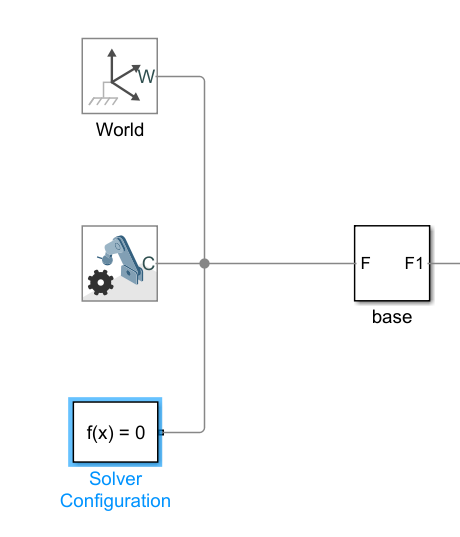
\includegraphics[width=6cm]{figures/r3.png}
			\caption{模型输入部分}\label{Fig_ro3}
		\end{minipage}%
		\begin{minipage}[t]{0.4\linewidth}
			\centering
			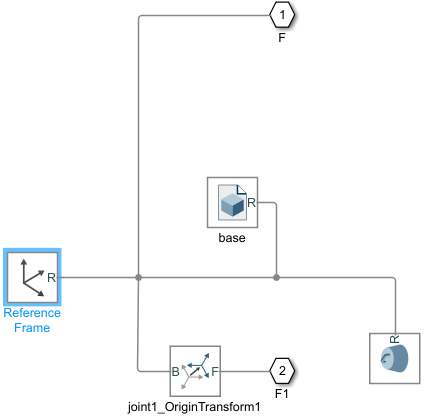
\includegraphics[width=6cm]{figures/r4.png}
			\caption{基座的坐标系与变换}\label{Fig_ro4}
		\end{minipage}%
\end{figure}

%\insertfig{./figures/r4.png}{基座的坐标系与变换}{Fig_ro4}{6cm}
\insertfig{./figures/r5.png}{基座模型}{Fig_r5}{5cm}

后续的每个连杆坐标系配置也是如此，不同的是往后坐标系变换更为复杂。坐标系要进行依次连乘，使得每个坐标系都能在世界坐标系下得到正确描述，如图(\ref{Fig_ro6})为第6连杆的配置。
\insertfig{./figures/r6.png}{连杆6的坐标系与变换}{Fig_ro6}{14cm}

为了机械臂能整体运动，还要将连杆通过关节相连，如图(\ref{Fig_ro7})为系统中关节1的截取图。仿真中的每一个关节单元都有两类输入和输出，第一类是坐标系的姿态，第二类是关节值、关节速度和关节加速度。如图(\ref{Fig_ro8})是关节1的输入部分，关节值以及它的一阶、二阶导数通过速率传输器一起输入到关节1。在经过函数变换后输出实际关节角度、角速度和角加速度（图\ref{Fig_ro9})。其余关节的配置也是如此。在整体上，为了保证各个关节的输入与输出的关系，对输入量与输出量的端口进行配置，如图(\ref{Fig_ro1})\par
\insertfig{./figures/r7.png}{关节1将基座与连杆进行连接}{Fig_ro7}{5cm}
\begin{figure}[H] %[H]让图片在文章中的位置就是这段代码的位置
	\centering
		\begin{minipage}[t]{0.4\linewidth}
			\centering
			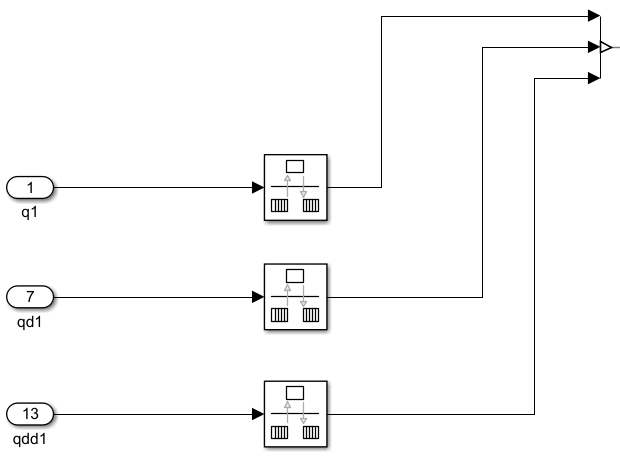
\includegraphics[width=6cm]{figures/r8.png}
			\caption{关节1的关节输入部分}\label{Fig_ro8}
		\end{minipage}%
		\begin{minipage}[t]{0.4\linewidth}
			\centering
			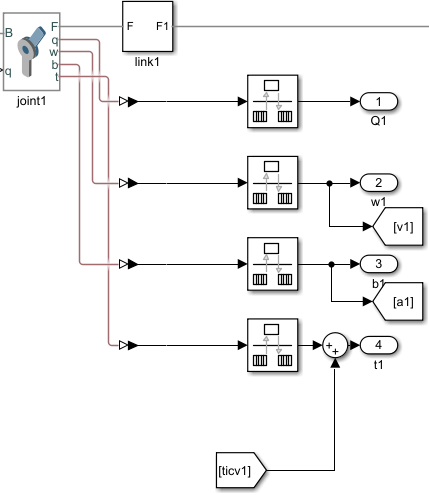
\includegraphics[width=6cm]{figures/r9.png}
			\caption{关节1的关节输出部分}\label{Fig_ro9}
		\end{minipage}%
\end{figure}
%\insertfig{./figures/r8.png}{关节1的关节输入部分}{Fig_ro8}{5cm}
%\insertfig{./figures/r9.png}{关节1的关节输出部分}{Fig_ro9}{5cm}
\insertfig{./figures/ro1.png}{关节输入输出端口转换}{Fig_ro1}{10cm}
配置完成后，可以在MATLAB的窗口看到该仿真机械臂的模型图（图\ref{Fig_simumani})。
\insertfig{./figures/simumani.png}{机械臂模型图}{Fig_simumani}{8cm}

\subsection{控制器设计}
\insertfig{./figures/ctr.png}{制作力位混合控制器}{Fig_ctr}{12cm}
控制器是控制系统的核心，进行机器人参数配置，调节系统的控制周期为1ms,设计仿真环境中的PID控制器，在位置控制方面，为了得到期望位置在末端坐标系下的描述，根据D-H参数编写基坐标系到工具坐标系的末端执行器的传递关系得到位置控制规律。用PID算法得到力控制规律，并且优化了当输入期望力为阶跃信号时的情况，因为此时在起始控制时刻会产生较大的期望位置偏移，造成无法求解逆运动学，或机器人起始速度非0，即初始加速度为无穷大，导致真实世界中机器人无法正常运动。所以采用了多项式插值方式求期望力，保证期望力连续改变。之后将两者通过选择矩阵S或者S'选择位置控制规律或力控制规律，然后使用逆运动学求解函数进行关节角度的求解。\par

\section{力位混合控制实验与结果}
本文的实验选择在$xoy$平面上进行位置控制，垂直于$xoy$平面上有位置约束，进行力控制。
\subsection{固定点的力位混合控制}
首先进行在固定点测试设计的力/位置混合控制算法的实验，然后再从静态扩展到动态的情况。\par
\insertfig{./figures/pinput.png}{位置输入详细图}{Fig_pinput}{12cm}
在本实验中，第一个控制任务是使机械臂的末端执行器在固定点，对接触面输出作用力$F_d$=$[0,-100]^T$(N)。根据任务需求，将正弦信号源(图\ref{Fig_pinput})设置为零输出，将阶跃信号源设置为输入源，设定阶跃时间为0.1$s$，幅值为0.2。将关节值设置为[0,0,0,0,0.25,0]。位置信号转换为如下阶跃信号。\par
\insertfig{./figures/pointr.png}{相对于基坐标系的阶跃输入}{Fig_pointr}{10cm}
\insertfig{./figures/pointx.png}{机械臂末端运动曲线}{Fig_pointx}{10cm}
可以看到在t=0.125s时达到稳态。机械臂末端的运动轨迹为(图\ref{Fig_pointx})
可以看出系统能较好的跟踪输入的阶跃信号。末端与表面的接触力变化曲线为(图\ref{Fig_pointf})\par
\insertfig{./figures/pointf.png}{固定点接触力变化曲线}{Fig_pointf}{10cm}
在严苛的阶跃信号输入下，接触力刚开始有一个很大的误差突变，在控制器的调节下，系统很快能减小误差，并且使接触力输出保持恒定，最终在-99.2N，稳态误差为0.8N。


\subsection{沿圆弧的力位混合控制}
在本小节中，使机械臂的执行器末端沿着圆弧运动，并对接触面施加恒定的接触力$F_d$=$[0,-100]^T$(N)。为了使机械臂把阶跃信号源的输出设置为零，把正弦信号设置为输入源。将关节值设置为[0,0,0,0,1,0]，在经过前向运动学的变换后，位置信号变为如下正弦波输入到控制器中：(图\ref{Fig_arcr})\par
\insertfig{./figures/arcr.png}{相对于基坐标系的正弦输入}{Fig_arcr}{10cm}
最后机械臂末端的运动轨迹为(图\ref{Fig_arcx})
\insertfig{./figures/arcx.png}{机械臂末端运动曲线1}{Fig_arcx}{10cm}
可以看出系统能较好的跟踪输入的正弦信号。末端与表面的接触力变化曲线为\par
\insertfig{./figures/arcf.png}{沿圆弧接触力变化曲线1}{Fig_arcf}{10cm}
在t$\textless$1s时，接触力变化缓慢，在1s$\textless$t$\textless$9s时，力误差开始快速收敛。系统最终的输出接触力大约为-100.2N，存在-0.2N的接触力误差(图\ref{Fig_arcf})。\par
将关节值保持不变，将期望接触力设置为$F_d$=$[0,-50]^T$(N)，机械臂末端运动曲线和接触力变化分别为：
\insertfig{./figures/arcx50.png}{机械臂末端运动曲线2}{Fig_arcx50}{10cm}
\insertfig{./figures/arcf50.png}{沿圆弧接触力变化曲线2}{Fig_arcf50}{10cm}
\section{小结}
本章对机械臂进行仿真实验，用PID方法设计控制器，并验证系统在不同任务下的表现。仿真实验过程中，机械臂轨迹平滑，跟踪精度较高。实验表明机械臂可以输出较准确的位置与接触力，验证了力/位置混合控制算法的有效性。
	
	%\newpage
\chapter{总结与展望}
\section{研究总结}
运动控制和力控制是机器人控制中主要的两个方面，过去机器人往往只要完成位置控制任务，而如今机器人往往需要完成更复杂更困难的任务，纯粹的位置控制已经满足不了这些需求。同时任务环境的恶劣性，使机械臂从结构上得到升级，促进了冗余机械臂的产生。冗余机械臂比起非冗余机械臂有更好的灵活性，但是对其进行控制也更困难。于是本文设计了对于冗余机械臂的力-位混合控制系统，本文主要工作如下：\par
(1)本文首先对冗余机械臂模型进行分析，用D-H参数法对冗余机械臂进行运动学建模，得到不同坐标系下的位姿关系。使用拉格朗日法进行动力学建模，求解了驱动机械臂关节运动需要的力矩。并且计算了雅可比矩阵使得直角坐标系下的位置和关节空间的角度之间，末端执行器与外界接触力与关节力矩之间的关系得到对应。实现了控制量与被控量的转换。仿真结果表明，模型能较准确的反映真实物理世界的机械臂。\par
(2)研究了力位混合控制算法，设计了PID控制器。将控制问题解耦为力控制子空间和位置控制子空间，实现某一自由度上不同方面的控制。
\section{工作展望}
冗余机械臂的力-位置混合控制在机器人应用中占据着重要地位，必然会得到更广泛深入的研究，一个优秀的控制系统是机器人完成任务的前提。本文针对冗余机械臂的特性设计了控制系统，从模型构建、控制算法理论分析和仿真研究等方面展开了研究，这些研究还有可以改进和深入之处:\par
(1)本文采用的PID控制器采用线性反馈性质，直接控制关节输出驱动力矩，虽然能比较准确地进行控制，但是机器人具有分线性和时变性，这使得控制效果还是存在一定误差，可以根据控制经验，使用模糊PID控制或者用非线性控制器例如循环神经网络等原理进行控制，会使控制精度得到提高。仍然需要通过大量的理论探索和实际应用对其进行完善。\par
(2)假如对于机械臂的姿态有指定要求，或者需要机械臂对环境施加力矩，那么该六自由度机械臂就达不到冗余的条件，未来会选取七自由度甚至更高自由度机械臂进行冗余的力位混合控制研究。\par
(3)本文的验证工作是通过仿真进行，然而实际的机器人关节机构存在反向间隙，有摩擦力干扰，反馈回路的传感器也存在噪声干扰，因此实际中，控制系统的设计还需要考虑系统对于干扰的鲁棒性。
	\newpage
%---------------------acknowledgement----------------%
	\addcontentsline{toc}{chapter}{致谢}
	\markboth{致谢}{}
	\begin{center}
		\textbf{\fontsize{16}{18}\selectfont 致\ \ 谢}
	\end{center}

	毕业设计的过程艰辛与痛苦交织，而在完成论文的现在心中却没有想象中的那么喜悦，反而怅然若失。四年的时光如白驹过隙，从大一入学开始学习一门门课程，参加一次次竞赛，整个大学四年一直从一座山丘翻越到下一座山丘，如今越过这些山丘的我才发现自己真的要与美好的大学四年生活说再见了。现在我想感谢一路上所有帮助我、关心我的人，没有你们，我也不可能成为现在的我。\par
    首先我要感谢师长，是你们一步步带我领略控制之美，让我从稀里糊涂选择这个专业，到如今对这一伟大专业产生认同与喜爱。特别感谢洪伟老师，您在我被隔离时还特地关心我的学习情况，为我解答课程疑惑，之后每当我想要摆烂时，都会想到此事让自己“重回正轨”。特别感谢Amanda老师，您的课堂随和有趣、内容丰富，虽然只上了您一年的英语课，不过在您课堂上学到的英语学习方法与萌生的英语兴趣使我受益四年。最要感谢的是我的导师崔靖涵老师，第一次上你的课就让我大开眼界，您教授的内容让我收获颇丰，使我发自内心为自己是双控人而骄傲。还要感谢刘老师，感谢你们对我毕业设计工作付出的心血。\par
    我还要感谢陪伴我生活学习的同学朋友们，是你们让这段时光丰富多彩、一生难忘。特别感谢辛昊东，你一直以来的自律与勇毅是我学习的榜样。你对我的鼓励与帮助，纯粹又充满力量，让我能够勇往直前，穿过那段最迷茫与自疑的时光。\par
    我要感谢我的父母，无论在什么方面、什么时候，你们都是我最后的、最有力的依靠。我知道你们一直都在。\par
    最后，也感谢一下自己吧。大学四年充满内耗与挣扎，要不是你一直以来的努力与坚持，也不会有此刻短暂的春和景明。希望今后你能在求是园更刻苦努力。\par
	
	




	\newpage
	\addcontentsline{toc}{chapter}{参考文献}
	\bibliographystyle{gbt7714-numerical}
	\bibliography{refs.bib}
	

	
\end{document} 